\documentclass[tikz]{standalone}
\usepackage{pgfmath}
\usetikzlibrary{calc}
\begin{document}
	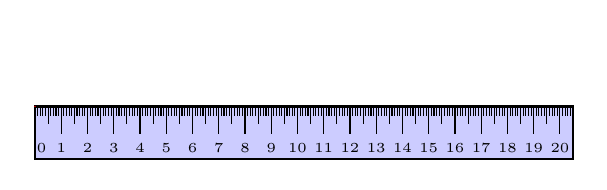
\begin{tikzpicture}[x=1cm,y=1cm]
		% Règle graduée : rectangle rempli en bleu avec graduation similaire
		\pgfmathsetmacro{\scaleRatio}{3} % longueur de la règle en cm
		\pgfmathsetmacro{\length}{20.5/\scaleRatio} % longueur de la règle en cm
		\pgfmathsetmacro{\height}{2/\scaleRatio}   % hauteur visuelle de la règle
		\pgfmathsetmacro{\tickMajor}{0.35}
		\pgfmathsetmacro{\tickMedium}{0.22}
		\pgfmathsetmacro{\tickMinor}{0.12}
		\pgfmathsetmacro{\labelgap}{0}

		% corps de la règle
		\coordinate (O) at (0,0);
		\fill[blue,fill opacity=0.2] (O) rectangle (\length,-\height);
		\draw[thick] (0,0) rectangle (\length,-\height);
		
		% graduations principales (tous les 1 unité) et étiquettes
		% graduations principales (tous les 1 cm) et étiquettes jusqu'à 20 cm
		\foreach \i in {0,...,20}{%
			\pgfmathsetmacro{\j}{\i/\scaleRatio}
			\draw[thin] (\j,0) -- (\j,-\tickMajor);
			% placer 0 avec ancrage à droite pour ne pas déborder
			\ifnum\i=0\relax
				\node[font=\tiny, below right, xshift=-0.1cm] at (\j,-\tickMajor-\labelgap) {0};
			\else
				\node[font=\tiny, below] at (\j,-\tickMajor-\labelgap) {\i};
			\fi
			}
			
		% graduations secondaires (tous les 0.5)
		% graduations secondaires tous les 0.5 cm (inclut 20.5)
		\foreach \j in {0,...,20}{%
			\pgfmathsetmacro{\x}{(\j+0.5)/\scaleRatio}
			\draw[thin] (\x,0) -- (\x,-\tickMedium);
		}
		
		% petites graduations (tous les 0.1 entre les unités, sauf aux majeures/mixtes)
		% petites graduations tous les 0.1 cm jusqu'à 20.5 cm (sauter 0.5)
		\foreach \k in {1,...,205}{%
			\pgfmathsetmacro{\x}{\k/10}
			% sauter les positions déjà dessinées (multiples de 0.5)
			\pgfmathparse{mod(\k,5)==0 ? 1 : 0}
			\ifnum\pgfmathresult=0\relax
				\draw[thin] (\x/\scaleRatio,0) -- (\x/\scaleRatio,-\tickMinor);
			\fi
		}
		\fill[opacity=0](0,0)--(1,0)--(0,1)--cycle;
		\fill[red,opacity=1] (O) circle (0.01);
	\end{tikzpicture}
	\end{document}